\begin{frame}{Introdução}
\begin{itemize}
\item Tecnologias computacionais auxiliam no processamento de dados
\ \ \newline
\item \alert{Meteorologia} é a ciência responsável pelo estudo do clima e tempo
\begin{itemize}
	\item Demanda por armazenamento, processamento e gerenciamento dos dados meteorológicos
	\item Necessidade  de confiabilidade e rapidez no processamento das informações
\end{itemize}
\end{itemize}
\end{frame}

\begin{frame}{Introdução}
\begin{itemize}
\item LabInstru: Laboratório de Instrumentação Meteorológica
\begin{itemize}
	\item Localizado na Escola Superior de Tecnologia (EST)
	\item Sala C29
	\item Universidade do Estado do Amazonas (UEA)
\end{itemize}
\ \ \newline
\item Administra a \alert{Estação Meteorológica Automática} da EST
\begin{itemize}
	\item Em funcionamento desde 2010
	\item Coleta de diversas variáveis meteorológicas
	\item Processamento e disponibilização dos dados
	\item Geração de boletins meteorológicos
\end{itemize}
\end{itemize}
\end{frame}

\begin{frame}{Introdução}
\begin{itemize}
\item Exemplo de arquivo-texto oriundo da estação meteorológica:
\end{itemize}

\begin{figure}
\centering
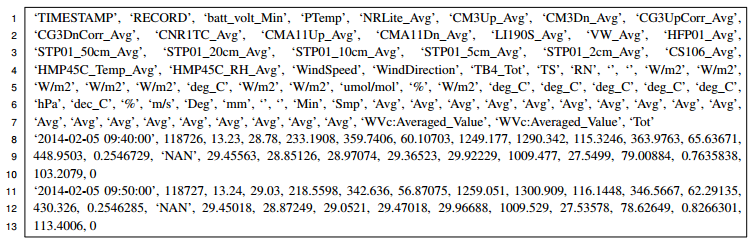
\includegraphics[width=0.9\linewidth]{./img/dat}
%\caption{Exemplo de um trecho dos dados encontrados no arquivo produzido pela estação meteorológica.} \label{fig:exemploBaixa1}
\end{figure}

\end{frame}

\begin{frame}{Introdução}

\begin{block}{Problemas Identificados}
	\begin{itemize}
		\item Processamento de dados feito de maneira manual
		\item Processo demorado e exaustivo
		\item Resultados sujeitos a erros e imprecisões
		\item Requer mão de obra especializada
	\end{itemize}
\end{block}
\ \ \newline

\end{frame}

\begin{frame}{Introdução}

\begin{block}{Objetivo Geral}
	\begin{itemize}
		\item Projetar e implementar uma plataforma web para armazenamento, gerenciamento e disponibilização de dados de uma estação meteorológica automática
	\end{itemize}
\end{block}
\ \ \newline

\begin{block}{Objetivos Específicos}
	\begin{itemize}
		\item Identificar e documentar as funcionalidades a serem desenvolvidas
		\item Elaborar protótipos de interface para validar as funcionalidades
		\item Levantamento das tecnologias utilizadas para o desenvolvimento da aplicação
		\item Projetar e implementar a plataforma web
		\item Implantar a plataforma web no LabInstru
	\end{itemize}
\end{block}
\ \ \newline

\end{frame}

\begin{frame}{Introdução}
\begin{block}{Metodologia}
	\begin{enumerate}
	\item Identificação de um processo de desenvolvimento
	\item Estudos dos arquivos gerados pela estação meteorológica
	\item Elicitação de requisitos
	\item Construção protótipos de interface gráfica
	\item Definição de uma agenda de implementação
	\item Identificação de tecnologias
	\item Implementação
	\item Escrita e defesa do TCC1
	\item Implantação
	\item Escrita e defesa do TCC2
\end{enumerate}
\end{block}


\end{frame}
